\chapter{RF-Score-v3: binding affinity prediction}

\section{Abstract}

There is a growing body of evidence showing that machine learning regression results in much more accurate structure-based prediction of protein-ligand binding affinity. Such prediction is a requirement for docking methods in that it is the basis for discriminating between active and inactive molecules or optimising the potency of a ligand against a target. However, despite their proven advantages, machine-learning scoring functions are still not widely applied. This seems to be due to insufficient understanding of their properties and the lack of user-friendly software implementing them.

Here we present a study where the accuracy of AutoDock Vina, arguably the most commonly-used docking software, is strongly improved by following a machine learning approach. We also analyse the factors that are responsible for this improvement and their generality. Most importantly, with the help of a proposed benchmark, we demonstrate that this improvement will be larger as more data becomes available for training Random Forest models, as regression models implying additive functional forms do not improve with more training data. We discuss how the latter opens the door to new opportunities in scoring function development. In order to facilitate the translation of this advance to enhance structure-based molecular design, we provide software to directly re-score Vina-generated poses and thus strongly improve their predicted binding affinity. The rescoring software is freely available at http://istar.cse.cuhk.edu.hk/rf-score-3.tgz.

This was a collaborative project with Pedro J. Ballester from Cancer Research Center of Marseille, Marseille, France. It was published in the \textit{Proceedings of the 11th International Meeting on Computational Intelligence Methods for Bioinformatics and Biostatistics (CIBB)} on 26 June 2014 \citep{1433}.

\section{Introduction}

Molecular docking is a key computational technique in structural bioinformatics and structure-based molecular design. Docking predicts the preferred conformations and binding strength of a ligand molecule, typically a small organic molecule, as bound to a protein pocket. Such prediction is necessary to discriminate between molecules that bind and those that do not bind to a target of interest (i.e. those molecules with high affinity for the target and those with an affinity so low that does not permit stable binding). Docking is not only useful to anticipate whether a ligand binds tightly to a target, but also to understand how it binds. The latter can be helpful to improve the potency and selectivity of binding.

Docking applications include, but are not limited to, structure-based virtual screening \citep{455,1383,1448}, drug lead optimisation \citep{1385}, polypharmacology prediction \citep{1449,1450}, drug repositioning \citep{1384}, binding pocket prediction \citep{384,1217}, human variation prediction \citep{1451}, protein function prediction \citep{1386} and target druggability assessment \citep{1472}.

Operationally, docking has two stages: predicting the position, orientation and conformation of a molecule when docked to the target's binding site (pose generation), and predicting how strongly the docked pose of such putative ligand binds to the target (scoring).  The single most important limitation of docking is the traditionally low accuracy of the scoring functions that predict the strength of binding.

Classical scoring functions assume a predetermined theory-inspired functional form for the relationship between the numerical features that describe the complex and its predicted binding affinity. There are three types of classical scoring functions: force-field \citep{1461,1462,959}, empirical \citep{1463,1464,1465,1466} and knowledge-based \citep{1467,1468,1469,1470}. Each type follows a different philosophical approach to scoring function development, as explained elsewhere, e.g. \citep{579}. However, it is important to note that these three types are mathematically equivalent in that a predetermined functional form is imposed to vertebrate the scoring function. In almost all classical scoring functions, the assumed functional form is additive. Furthermore, like empirical scoring functions, most modern force-field and knowledge-based scoring functions weight their constituent terms by fitting experimental binding data \citep{579}. Figure \ref{rfscore3:ClassicalScoringFunctions} illustrates the mathematical equivalence of these three popular classical scoring functions as sums of data-weighted energetic contributions to binding. $K_j$ is the total number of protein atoms of type $j$ and $L_i$ is the total number of ligand atoms of type $i$ in the considered complex. An atom type is defined according to atomic number and in some cases also using the calculated protonation state (e.g. hydrogen bond donors). The additive terms may additionally impose interatomic distance and angle constraints between neighbouring atoms of the considered types (e.g. hydrogen bonding terms).

\begin{figure}
\centering
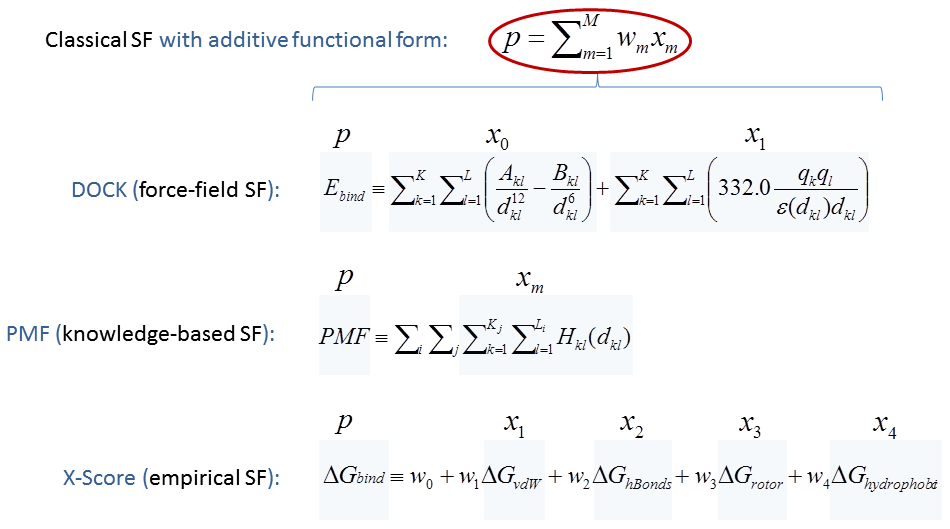
\includegraphics[width=\linewidth]{../rfscore3/ClassicalScoringFunctions.png}
\caption{Mathematical equivalence of classical scoring functions as sums of data-weighted energetic contributions to binding.}
\label{rfscore3:ClassicalScoringFunctions}
\end{figure}

Recently, machine-learning scoring functions have been shown \citep{564} to be much more accurate than classical scoring functions at binding affinity prediction. This improvement is due to two factors. The first is the circumvention of the assumed functional form of classical scoring functions, which is learnt instead in an entirely data-driven manner in machine-learning scoring functions. This was to be expected as it is well known that individual free energy terms may not be additive \citep{1471,1416}. Second, research on classical scoring functions has focused on increasingly detailed modelling of contributions to binding, but it has now been established that a more precise description of protein-ligand complexes does not generally lead to more accurate prediction of binding affinity \citep{1370}. This study has resulted in an expected set of structural descriptors leading to improved performance when allied with a sufficiently flexible regression model.

Machine-learning scoring functions have been misclassified as knowledge-based scoring functions \citep{1373,1372} or empirical scoring functions \citep{1305}, but these are fundamentally different from either type because of not imposing a fixed functional form on the relationship between structural and binding data. This distinction between machine-learning and classical scoring functions has important consequences in practice, as it will be analysed.

Despite being a recent development, there are already successful prospective applications of machine-learning scoring functions. RF-Score \citep{564} has recently been used \citep{1281} to discover a large number of innovative binders of antibacterial DHQase2 targets. To facilitate its use, RF-Score  has now been incorporated into a user-friendly large-scale docking web server for prospective virtual screening, available at http://istar.cse.cuhk.edu.hk/idock \citep{1362}. On the other hand, a machine-learning scoring function called MD-SVR has been generated and applied \citep{1452} to guiding the optimisation of known Akt1 kinase inhibitors. The derivatives highlighted by MD-SVR were synthesised and all of them exhibited moderate to good inhibitory activities.

This innovative methodology has however raised a few concerns. For example, the use of oversimplified features in the original version of RF-Score has been pointed out as problematic \citep{1453}, although no empirical evidence was provided in support of this claim and this version actually achieved high hit rates in prospective virtual screening \citep{1281}. The superior performance of RF-Score was highlighted by \citep{774}, which nevertheless attributed it to the characteristics of the most widely-used benchmark. This was subsequently demonstrated not to be the case \citep{908}. Still, there seem to be some concerns that the applicability domain of machine-learning scoring functions would be somehow more restrictive than that of classical scoring functions. Lastly, \citep{1372} claimed that the application of machine-learning scoring functions is limited by their tendency to overfit training data and their alleged difficulty in providing an immediate physical interpretation of the results.

In this paper, we show that one can construct a machine-learning scoring function from a classical scoring function to have the same applicability domain and interpretability capabilities while greatly improving its ability to predict binding affinity. This will be shown with AutoDock Vina \citep{595} as the classical scoring function because it is arguably very popular. Furthermore, we will also address the remaining criticisms supported by numerical experiments. Finally, the growing importance of machine-learning scoring functions will be demonstrated in the context of a purposely-built new benchmark by analysing how their performances improve with the increase of structural and binding data used for training.

\section{Methods and materials}

This section introduces four scoring functions building upon AutoDock Vina, two benchmarks to evaluate performance of these scoring functions and the performance metrics that will be used to this end.

\subsection{Model 1 - AutoDock Vina}

The AutoDock series \citep{597,596,595} is the most cited docking software by the research community, with over 8,000 citations to date between these three publications, according to Google Scholar. As the successor of AutoDock 4 \citep{596}, AutoDock Vina \citep{595} significantly improved the average accuracy of the binding mode predictions, while running two orders of magnitude faster with multithreading. Vina was an exciting development, not only because of its remarkable pose generation performance in terms of both effectiveness and efficiency, but also because it is an open source tool and is among the most accurate classical scoring functions for binding affinity prediction.

Like all classical scoring functions, Vina assumes a predetermined functional form. In this case, Vina's score for the $k$th conformer, $e_k$, is calculated as:

\begin{equation}
\label{rfscore3:e_k}
e_k=\frac{e_{k,inter}+e_{k,intra}-e_{1,intra}}{1+w_6N_{rot}}
\end{equation}

Now because studies on binding affinity prediction are benchmarked on co-crystallised ligands to avoid confounding factors, there is only one conformer per molecule ($k=1$) and thus the intramolecular contribution cancels out giving:

\begin{equation}
\label{rfscore3:e_1}
e_1=\frac{e_{1,inter}}{1+w_6N_{rot}}
\end{equation}

where

\begin{eqnarray}
\label{rfscore3:e_1_inter}
e_{1,inter} &=& w_1 \cdot Gauss1_1 \nonumber \\
            &+& w_2 \cdot Gauss2_1 \nonumber \\
		    &+& w_3 \cdot Repulsion_1 \nonumber \\
		    &+& w_4 \cdot Hydrophobic_1 \nonumber \\
		    &+& w_5 \cdot HBonding_1
\end{eqnarray}

\begin{equation}
\label{rfscore3:w}
\mathbf w=(-0.035579,-0.005156,0.840245,-0.035069,-0.587439,0.05846)
\end{equation}

$e_1$ is the predicted free energy of binding reported by the Vina software when scoring the structure of a protein-ligand complex. The values for the six weights were found by Ordinary Least Squares (OLS) using a nonlinear optimisation algorithm as it has been the case in related force-field scoring functions \citep{1454}, although this process was not detailed in the original publication \citep{595}. The training data was PDBbind v2007 refined set (N=1300). $N_{rot}$ is the number of rotatable bonds. Unlike other classical scoring functions, Vina is not exactly a sum of energy terms because $w_6\neq0$, although it is quasi-linear since $1+w_6N_{rot}$ takes values close to 1 for most protein-ligand complexes. As usual, e.g. \citep{1362}, the predicted free energy of binding in kcal/mol units is converted into pKd with $pK_d=-0.73349480509e_1$ in order to compare to binding affinities ($pK_d$ or $pK_i$). Expressions and further details for the five $e_{k, inter}$ terms can be found in \citep{595,1362}.

\subsection{Model 2 - MLR::Vina}

This is a multiple linear regression (MLR) model using the six unweighted Vina terms as features. The use of MLR as the regression model implies an additive functional form and hence MLR::Vina is a classical scoring function. It adopts the philosophy of empirical scoring functions.

In order to make the problem amenable to MLR, we made a grid search on the $w_6$ weight and thereafter ran MLR on the remaining five weights. Specifically, we sampled 101 values for $w_6$ from 0 to 1 with a step size of 0.01. Interesting we found that the $w_6$ values of the best models were always between 0.005 and 0.020. Then we again sampled 16 values for $w_6$ in this range with step size 0.001, and used the best of them in terms of the lowest RMSE (Root Mean Square Error) on the training set.

\subsection{Model 3 - RF::Vina}

While Vina's ability to predict binding affinity is among the best provided by classical scoring functions, it is still limited by the assumption of a functional form. To investigate the impact of this modelling assumption, we used Random Forest (RF) \citep{1309} to implicitly learn the functional form from the data. Other machine learning techniques can of course be applied to this problem, e.g. SVR (Support Vector Regression) \citep{1295}, although this is out of the scope of the study.

A RF is an ensemble of many different decision trees randomly generated from the same training data \citep{1309}. RF trains its constituent trees using the CART algorithm \citep{1310}. Instead of using all features, RF selects the best data split at each node of the tree from a typically small number (mtry) of randomly chosen features. In regression problems, the RF prediction is given by arithmetic mean of all the individual tree predictions in the forest.

Here we built a RF model with the six Vina features using the default number of trees (500) and values of the mtry control parameter from 1 to all 6 features. The selected model was that with the mtry value providing the lowest RMSE on a subset of training data known as the OOB (Out of Bag) data. This process was repeated ten times with ten different random seeds because RF is stochastic. Further details on RF model building in this context can be found in \citep{564}.

\subsection{Model 4 - RF::VinaElem}

This is the model described in the previous subsection with an expanded set of 42 features once the 36 RF-Score features are added to the six Vina features. For a given random seed, a RF for each mtry value from 1 to 42 was built and that with the lowest RMSE on OOB data was selected as the scoring function. Like in the training process of model 3, the same ten seeds were used.

To calculate RF-Score features, atom types were selected so as to generate features that are as dense as possible, while considering all the heavy atoms commonly observed in PDB complexes (C, N, O, F, P, S, Cl, Br, I). As the number of protein-ligand contacts is constant for a particular complex, the more atom types are considered, the sparser the resulting features will be. Therefore, we selected a minimal set of atom types by considering atomic number only. Furthermore, a smaller set of interaction features has the additional advantage of leading to computationally faster scoring functions.

RF-Score features are defined as the occurrence count of intermolecular contacts between elemental atom types $i$ and $j$, as shown in equations \eqref{rfscore3:x_ij} and \eqref{rfscore3:x}, where $d_{kl}$ is the Euclidean distance between the $k$th protein atom of type $j$ and the $l$th ligand atom of type $i$ calculated from a structure; $K_j$ is the total number of protein atoms of type $j$ ($\#\{j\}=9$) and $L_i$ is the total number of ligand atoms of type $i$ ($\#\{i\}=4$) in the considered complex; $H$ is the Heaviside step function that counts contacts within a $d_{cutoff}$ neighbourhood. For example, $x_{7,8}$ is the number of occurrences of protein oxygen atoms hypothetically interacting with ligand nitrogen atoms within a chosen neighbourhood. Full details on RF-Score features are available at \citep{564,1295}.

\begin{equation}
\label{rfscore3:x_ij}
x_{ij}=\sum_{k=1}^{K_j}\sum_{l=1}^{L_i}H(d_{cutoff}-d_{kl})
\end{equation}

\begin{equation}
\label{rfscore3:x}
\mathbf x=\{x_{ij}\}\in N^{36}
\end{equation}

\subsection{The PDBbind benchmark}

Using predefined training and test sets, where other scoring functions had previously been tested, has the advantage of minimising the risk of using a benchmark complementary to the presented scoring function. There are many examples of benchmarks to validate generic scoring functions \citep{1455,1456,571,1457}.

Here we use the PDBbind benchmark \citep{1313}, arguably the most widely used for binding affinity prediction of diverse complexes. This benchmark is based on the 2007 version of the PDBbind database, which contains a particularly diverse collection of 1300 protein-ligand complexes with their corresponding binding affinities, assembled through a systematic mining of the entire PDB (Protein Data Bank) \citep{540,537}.

The PDBbind benchmark essentially consists of testing the predictions of scoring functions on the 2007 core set, which comprises 195 diverse complexes with measured binding affinities spanning more than 12 orders of magnitude, while training in the remaining 1105 complexes in the refined set. In this way, a set of protein-ligand complexes with measured binding affinity can be processed to give two non-overlapping data sets, where each complex is represented by its feature vector $\mathbf x_i$ and its binding affinity $y_i$, which includes both pKd and pKi measurements, henceforth referred to as just pKd for simplicity:

\begin{equation}
\label{rfscore3:D_train}
D_{train}=\{y_i,\mathbf x_i\}_{i=1}^{1105}
\end{equation}

\begin{equation}
\label{rfscore3:D_test}
D_{test}=\{y_i,\mathbf x_i\}_{i=1106}^{1300}
\end{equation}

\begin{equation}
\label{rfscore3:y}
y=pK_d=-\log_{10}K_d
\end{equation}

This benchmark has the advantage of permitting a direct comparison against the performance of 16 classical scoring functions that had previously been benchmarked on the same test set \citep{1313}. These 16 classical scoring functions include five scoring functions in the Discovery Studio software version 2.0 from Accelrys: LigScore \citep{1466}, PLP \citep{1467}, PMF \citep{1468}, Jain \citep{1473} and LUDI \citep{1463}, five scoring functions (D-Score, PMF-Score, G-Score, Chem-Score, and F-Score) in the SYBYL software version 7.2 from Tripos, GlideScore \citep{1465} in the Schrödinger software version 8.0 from Schrödinger, three scoring functions in the GOLD software version 3.2 from the CCDC: GoldScore \citep{1474}, ChemScore \citep{1464} and ASP \citep{1469}, and two standalone scoring functions released by academic groups: DrugScore \citep{1470,1475} and X-Score version 1.2 \citep{573}. Several of these scoring functions had different versions or multiple options, including LigScore (LigScore1 and LigScore2), PLP (PLP1 and PLP2), and LUDI (LUDI1, LUDI2, and LUDI3) in Discovery Studio; GlideScore (GlideScore-SP and GlideScore-XP) in the Schrödinger software; DrugScore (Drug-ScorePDB and DrugScoreCSD); and X-Score (HPScore, HMScore, and HSScore). For simplicity, the authors who tested all these scoring functions on the PDBbind benchmark \citep{1313} only reported the best performance of the version/options of each scoring function. Furthermore, we added to the comparison other classical scoring functions that have subsequently been tested on this benchmark: IMP::RankScore \citep{987} in \citep{1370}, HYDE2.0::HbondsHydrophobic \citep{1458}, PHOENIX \citep{576}, Cyscore \citep{1372}, HotLig \citep{1459} and DSX\textsuperscript{CSD} \citep{1460}. Many machine-learning scoring functions have also been tested on this benchmark, which are however not relevant for the goals of this study and hence not included.

\subsection{The 2013 blind benchmark}

We propose a new benchmark mimicking a blind test to provide a more realistic validation than the PDBbind benchmark, where higher performance is to be expected due to the protocol that generates this partition \citep{908}. The new test set comprises all the structures in the 2013 release of the PDBbind refined set that were not already in the 2012 release, i.e. the new 382 protein-ligand complexes added in 2013, whereas the 2012 refined set is used for training. This is hence conducted as a blind test in that only data available until a certain year is used to build the scoring function that predicts the binding affinities of 2013 complexes as if these had not been measured yet.

In addition, we define three more training sets to account for the structural and binding data available in the public domain at three previous times. These three previous PDBbind releases were selected so that there is approximately the same number of complexes between consecutive releases. In this way, one can use these four partitions sharing the same test set to study how scoring function performance varies with training data set size.

Table \ref{rfscore3:partitions} shows the data partitions. Partition 1 is the PDBbind benchmark. Refined02 means the 2002 release of the PDBbind refined set, whereas refined07$\backslash$core07 means the complexes left in refined07 after removing those in core07. By construction of each partition, there are no complexes in common between any training set and test set pair. In other words, there is no overlap between both sets and hence each test set complex is new data not seen in model training. Note that only models 2, 3 and 4 were re-trained on each of the five training sets, whereas model 1, AutoDock Vina, was used out of the box without re-training.

\begin{table}
\caption{Data set partitions of the 2013 blind benchmark.}
\label{rfscore3:partitions}
\begin{tabular}{clrlr}
\hline
Partition & Training set & N & Test set & N\\
\hline
1 & refined07$\backslash$core07 & 1105 & core07                         & 195\\
2 & refined02                   &  792 & refined13$\backslash$refined12 & 382\\
3 & refined07                   & 1300 & refined13$\backslash$refined12 & 382\\
4 & refined10                   & 2059 & refined13$\backslash$refined12 & 382\\
5 & refined12                   & 2897 & refined13$\backslash$refined12 & 382\\
\hline
\end{tabular}
\end{table}

One may argue that an additional partition is necessary, where all training complexes similar to any of the test complexes in some way are removed. Nevertheless, in practice, a test set will contain really few complexes of this type. Therefore, we would be depriving the scoring functions of the most relevant training data, which would actually be available, without good reason, leading to unrealistically low performance for all scoring functions. This point has already been discussed elsewhere \citep{908,1432}.

\subsection{Performance measures}

As usual \citep{1313}, performance will be measured by the Standard Deviation (SD), Root Mean Square Error (RMSE), Pearson correlation (Rp) and Spearman rank-correlation (Rs) between predicted and measured binding affinity. SD is included to permit comparison to previously-tested scoring functions on this benchmark. RMSE, on the other hand, reflects the ability of the scoring function to report an accurate binding affinity value. Rs shows how well it can rank bound ligands according to binding strength. Rp simply shows how linear the correlation is and thus it is a less relevant indicator of the quality of the prediction. The mathematical expressions of these four metrics can be found in \citep{1432}.

\section{Results and discussion}

Figures \ref{rfscore3:partition1stat} and \ref{rfscore3:partition5stat} show the predictive performance of the four models on the PDBbind benchmark (partition 1 in Table \ref{rfscore3:partitions}) and the 2013 blind benchmark (partition 5 in Table \ref{rfscore3:partitions}), respectively.

\begin{figure}
\centering
\subfloat[AutoDock Vina.]
{
  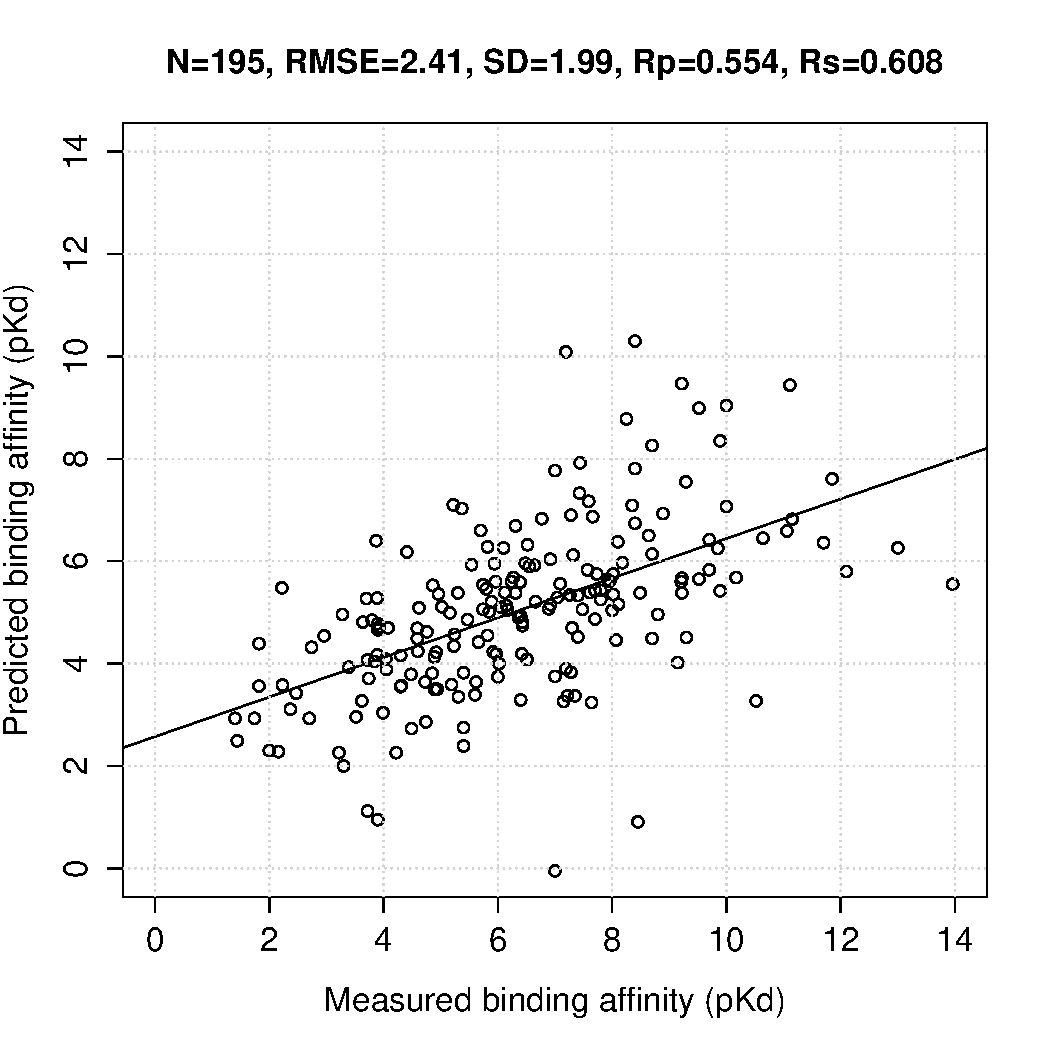
\includegraphics[width=0.48\linewidth]{../rfscore3/model-1-set-1-pdbbind-2007-tst-yp.pdf}
}
\subfloat[MLR::Vina.]
{
  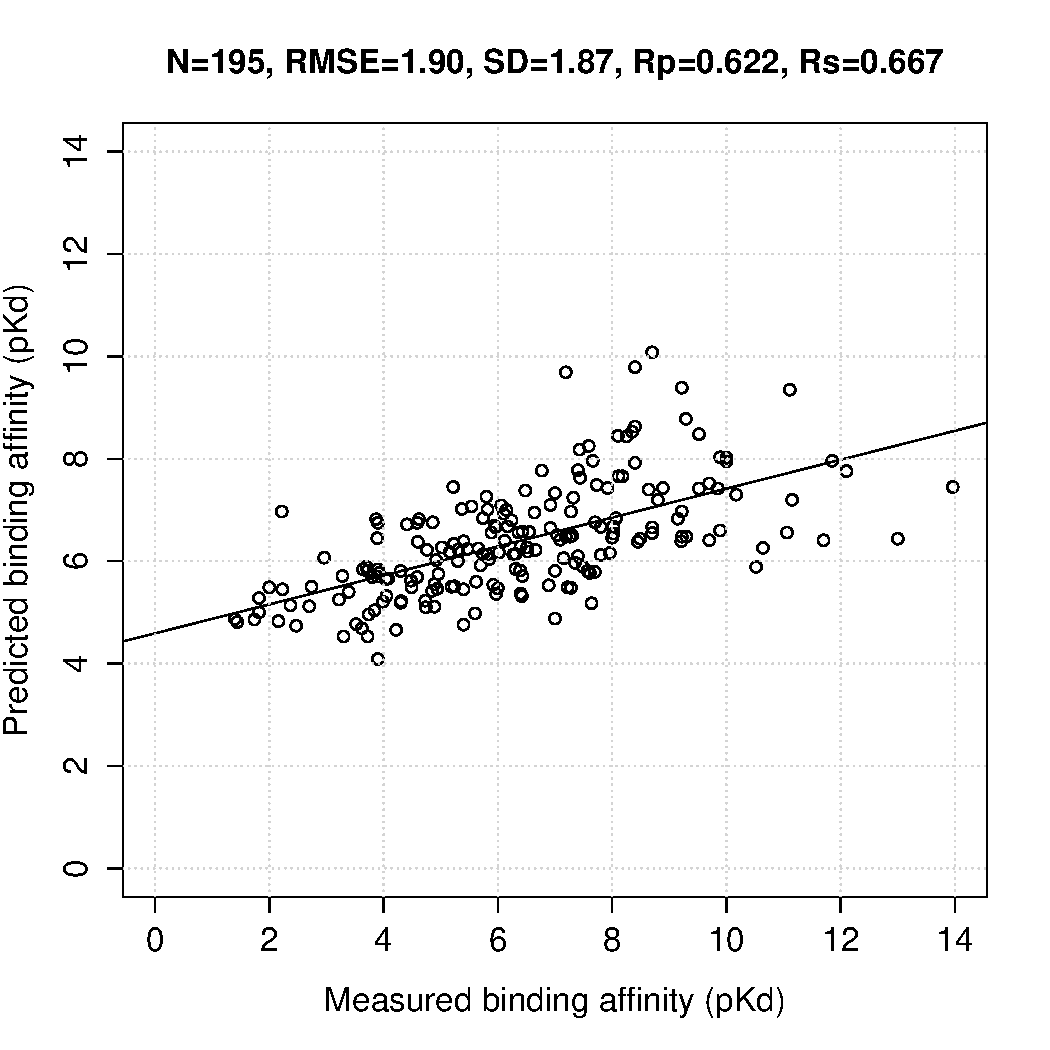
\includegraphics[width=0.48\linewidth]{../rfscore3/model-2-set-1-pdbbind-2007-tst-yp.pdf}
}
\\
\subfloat[RF::Vina.]
{
  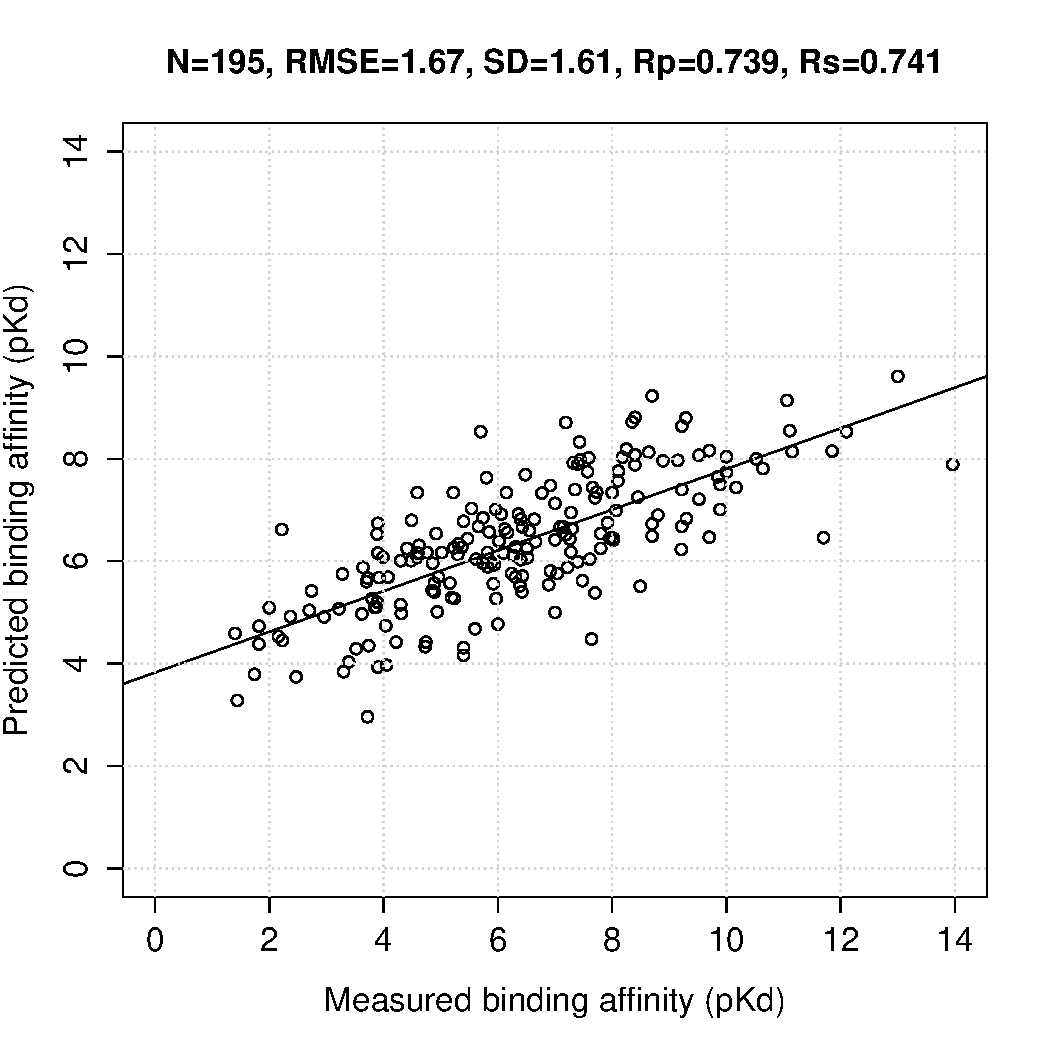
\includegraphics[width=0.48\linewidth]{../rfscore3/model-3-set-1-pdbbind-2007-tst-yp.pdf}
}
\subfloat[RF::VinaElem.]
{
  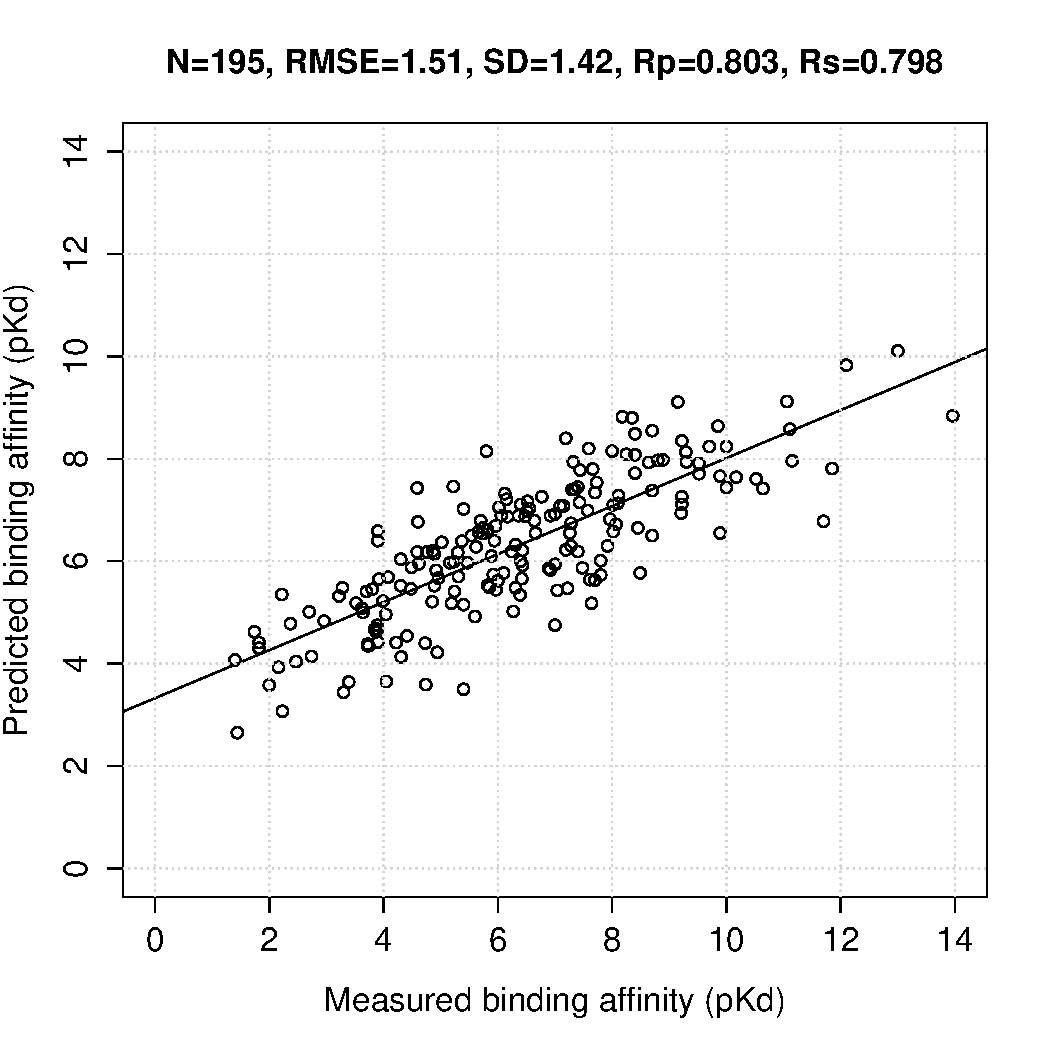
\includegraphics[width=0.48\linewidth]{../rfscore3/model-4-set-1-pdbbind-2007-tst-yp.pdf}
}
\caption{Performance on the 195 test set complexes in the PDBbind benchmark.}
\label{rfscore3:partition1stat}
\end{figure}

\begin{figure}
\centering
\subfloat[AutoDock Vina.]
{
  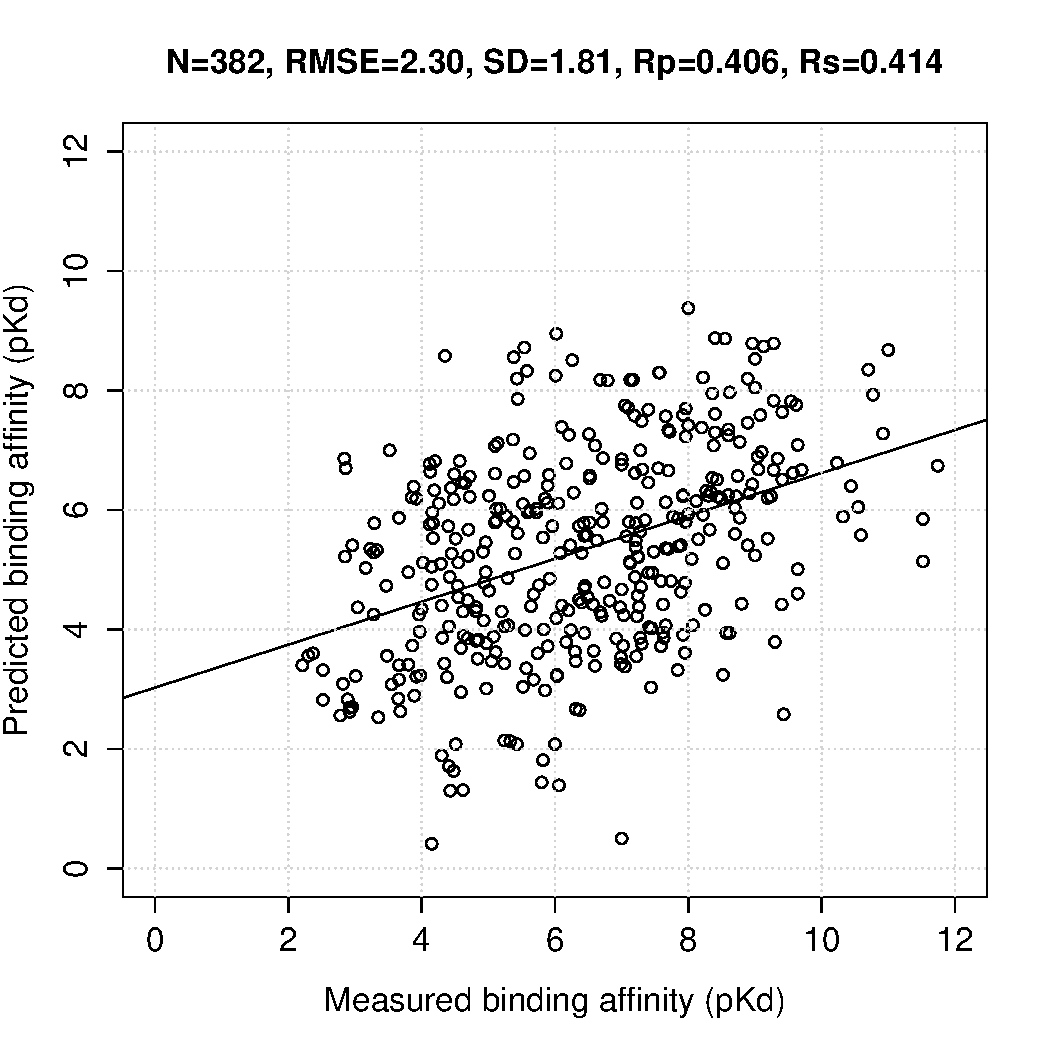
\includegraphics[width=0.48\linewidth]{../rfscore3/model-1-set-2-pdbbind-2007-tst-yp.pdf}
}
\subfloat[MLR::Vina.]
{
  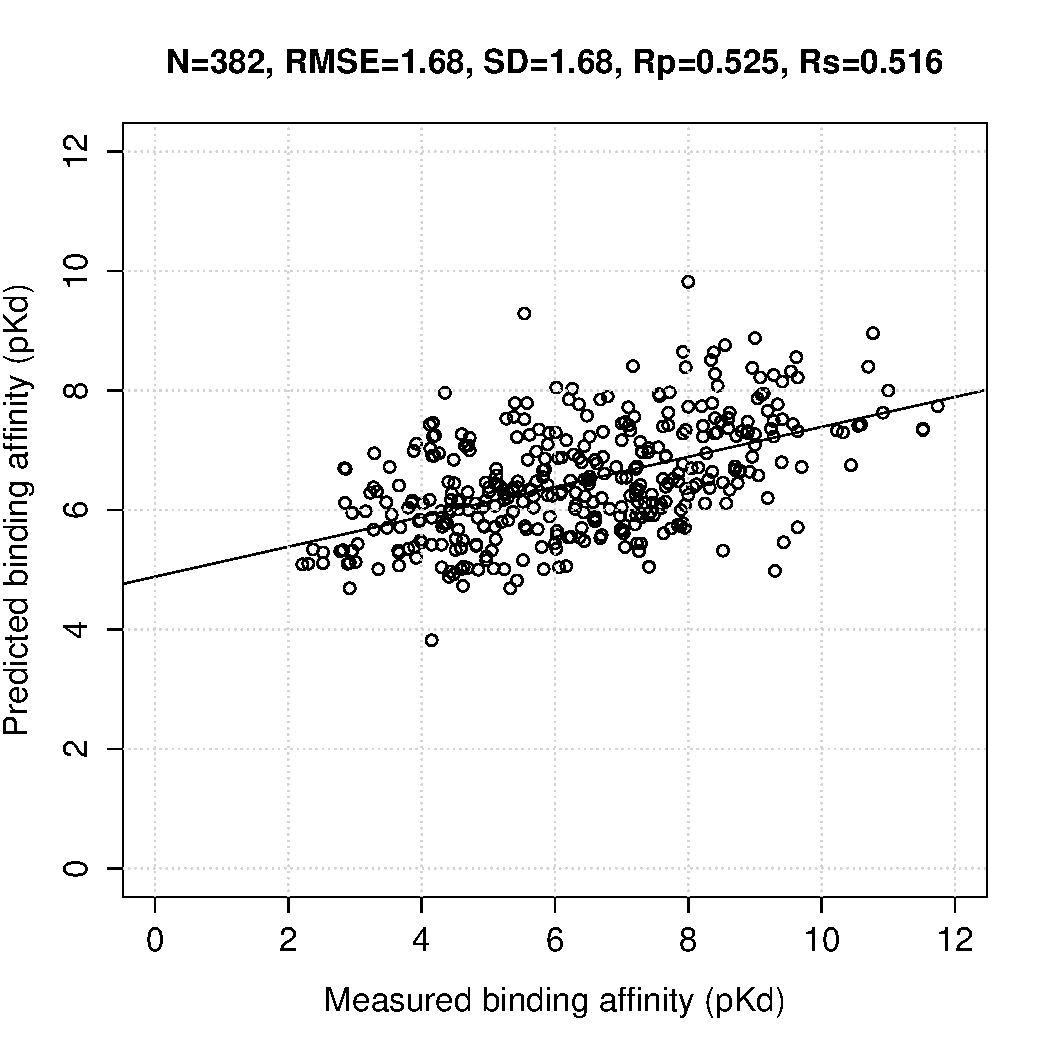
\includegraphics[width=0.48\linewidth]{../rfscore3/model-2-set-2-pdbbind-2012-tst-yp.pdf}
}
\\
\subfloat[RF::Vina.]
{
  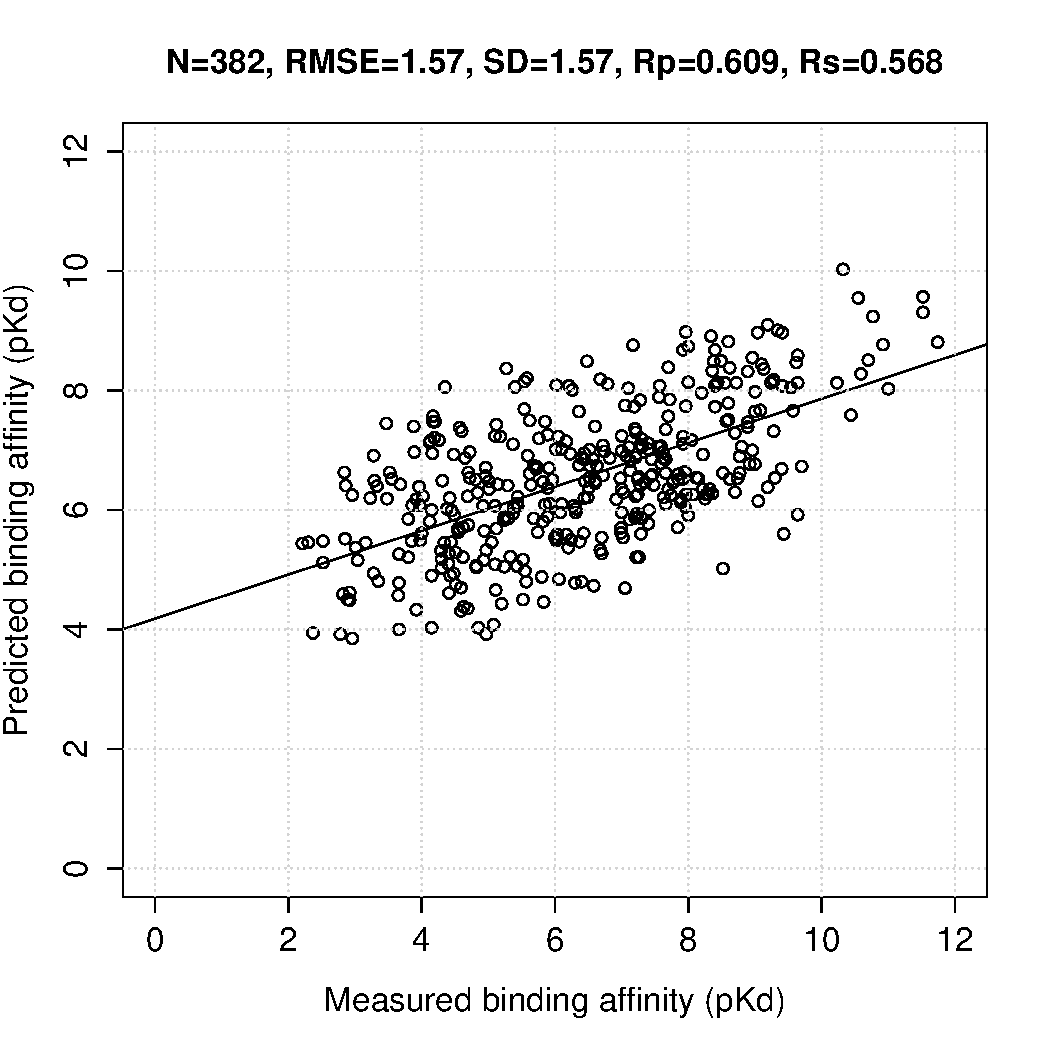
\includegraphics[width=0.48\linewidth]{../rfscore3/model-3-set-2-pdbbind-2012-tst-yp.pdf}
}
\subfloat[RF::VinaElem.]
{
  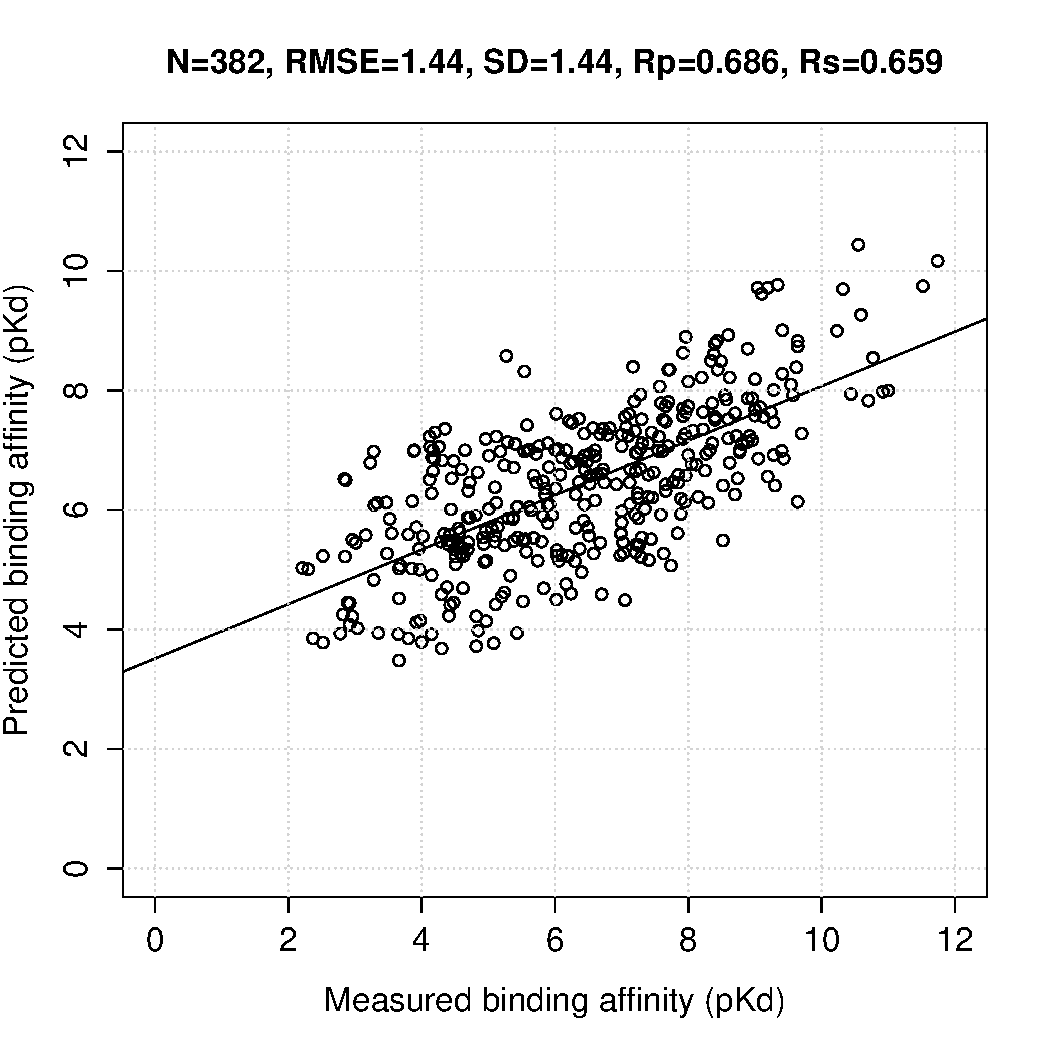
\includegraphics[width=0.48\linewidth]{../rfscore3/model-4-set-2-pdbbind-2012-tst-yp.pdf}
}
\caption{Performance on the 382 test set complexes in the 2013 blind benchmark.}
\label{rfscore3:partition5stat}
\end{figure}

\subsection{MLR is better at calibrating the additive functional form of Vina's scoring function}

Figures \ref{rfscore3:partition1stat} and \ref{rfscore3:partition5stat} show that MLR::Vina provided a test set performance with significantly lower error and higher correlation than Vina on both benchmarks. This means that MLR is more suitable to calibrate Vina's scoring function than the originally used nonlinear optimisation algorithm.

\subsection{Vina's assumed functional form is detrimental for its performance}

Both the linear (model 2) and nonlinear (model 1) optimisation approaches to training Vina assume a quasi-additive functional form. By looking at Figures \ref{rfscore3:partition1stat} and \ref{rfscore3:partition5stat}, it is clear that model 3 performed much better than models 1 and 2. Note that model 3 uses exactly the same features as the other two models, and it uses exactly the same training data as model 2. The only difference between these models is that model 3 implicitly constructs the functional form from the data using RF for regression, whereas the other two Vina models assume a priori form for how the features are combined to form the scoring function. Therefore, these results demonstrate that this performance improvement is entirely due to the avoidance of this commonly-used modelling assumption.

\subsection{Incorporating ligand properties increases performance further}

$N_{rot}$, unlike the remaining five fixed Vina features, which encode properties of the protein-ligand complex, is exclusively a property of the ligand. It is the number of rotatable bonds, effectively an estimation of the flexibility of the ligand. When model 3 was run with five features (all but $N_{rot}$), test set error increased from a best RMSE of 1.67 to 1.74, and Rs correlation dropped from 0.739 to 0.706 on the PDBbind benchmark. This result shows that it is advantageous to add $N_{rot}$ as a model feature. More broadly, this suggests that incorporating ligand properties into the model, such as those that are routinely used in ligand-based QSAR models, may enhance performance further. Likewise, features encoding protein properties could also extend the capabilities of generic scoring functions.

\subsection{The impact of overfitting on RF performance}

It has been recently claimed \citep{1372} that the tendency of machine-learning scoring functions to overfit training data is a weak point limiting their application. This is a surprisingly common misconception, whereby a less overfitted model is regarded as necessarily better than a more overfitted model. The latter implicitly assumes that the impact of overfitting will be the same for different classes of regression models. Nevertheless, some models, e.g. RF, are robust to overfitting in the sense that this has a low impact on its generalization ability.

To quantify the impact of overfitting, we trained MLR::Vina and RF::Vina on the same 1105 complexes and use them to predict the binding affinity of the 195 test set complexes in partition 1 in Table \ref{rfscore3:partitions}. MLR::Vina performed better on the training set than on the test set (SD=1.73 vs SD=1.87, respectively), which suggests that classical scoring functions only have a small degree of overfitting. In contrast, RF::Vina's performance was much better on the training set than on the test set (SD=0.60 vs SD=1.61, respectively), which evidences that RF significantly overfits training data. However, the large performance gain of RF::Vina over MLR::Vina on the test set (SD=1.61 vs SD=1.87, respectively) makes clear that RF::Vina is substantially more accurate than MLR::Vina regardless of overfitting. Therefore, overfitting cannot be used to anticipate the relative performance of two different models on a test set and hence it is necessary to measure the true impact of overfitting on the compared models.

Next, we used partition 5 from Table \ref{rfscore3:partitions} to provide further evidence that overfitting is not a weak point limiting the application of RF-based scoring functions. The training set is composed of 2897 complexes and test set is composed of 382 complexes, which as that from partition 1 also contains complexes that are very different among themselves. The test set was subdivided into five equally-sized new sets and the operation was repeated ten times to provide 50 different smaller test sets with 76 or 77 complexes each. Thereafter, we evaluated MLR::Vina and RF::VinaElem on each test set and plotted the resulting SD errors in Figure \ref{rfscore3:Models24SD}. If overfitting was a problem with RF, a highly variable difference in performance between both models would have been observed, with the less overfitted model being often better than the more overfitted model. By contrast, not once MLR::Vina outperformed RF::VinaElem. 

\begin{figure}
\centering
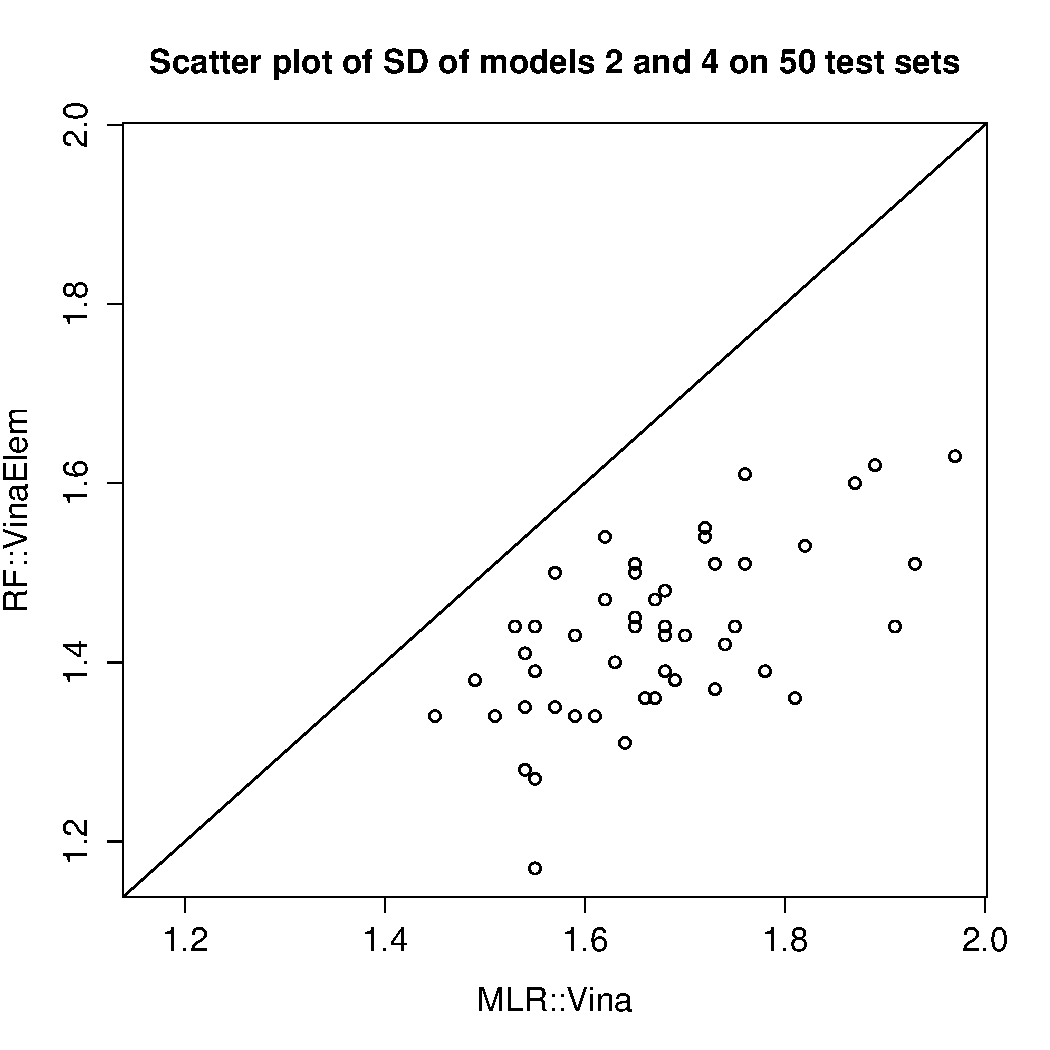
\includegraphics[width=\linewidth]{../rfscore3/Models24SD.pdf}
\caption{MLR::Vina and RF::VinaElem, both trained on the same 2897 complexes, compared on 50 test sets by their SD errors.}
\label{rfscore3:Models24SD}
\end{figure}

\subsection{Improvement of AutoDock Vina using RF}

RF::VinaElem is the product of two improvements over Vina: using RF on the six Vina features to circumvent the need of a functional form (model 3) and combining the latter with an expanded set of 42 features incorporating the 36 RF-Score features (model 4). Figure \ref{rfscore3:partition1stat} clearly shows that RF::VinaElem greatly improved Vina by -0.90 in RMSE, -0.57 in SD, +0.249 in Rp and +0.190 in Rs. In comparison, the NHA baseline obtained RMSE=2.15, SD=2.15, Rp=0.431, Rs=0.510, and the MWT baseline obtained RMSE=2.16, SD=2.17, Rp=0.418, Rs=0.496.

Figure \ref{rfscore3:partition5stat} also shows the same conclusion, with RF::VinaElem also achieving a substantial improvement over Vina of -0.86 in RMSE, -0.37 in SD, +0.280 in Rp and +0.245 in Rs. While there is a significant decrease in Rp and Rs for both scoring functions with respect to the PDBbind benchmark (compare Figures \ref{rfscore3:partition1stat} and \ref{rfscore3:partition5stat}), the relative performance of both scoring functions is similar on both benchmarks as it was anticipated \citep{908}. In comparison, the NHA baseline obtained RMSE=1.90, SD=1.89, Rp=0.295, Rs=0.363, and the MWT baseline obtained RMSE=1.90, SD=1.90, Rp=0.269, Rs=0.330.

On the other hand, it is well known that there is a considerable correlation between ligand size and binding affinity. Thus, simple models such as the MWT baseline have been used to put in perspective the performance of scoring functions. Table \ref{rfscore3:trn1105tst195} shows that many classical scoring functions are close to or even below this simple baseline. By contrast, RF::VinaElem obtained an Rp of 0.803 on the PDBbind benchmark, which almost doubles that of MWT (0.418). On the 2013 blind benchmark, RF::VinaElem obtained a Rp of 0.686 whereas MWT's was just 0.269. This is not surprising as RF::VinaElem has been designed to learn the relationship between intermolecular interactions and binding affinity from structural data, not ligand properties, which were solely used in the NHA and MWT baselines.

Overall, it is remarkable that RF::VinaElem achieved an error of just 1.44 pKd units, or 1.96 kcal/mol equivalently, in a blind benchmark comprising such a diverse independent test set (Figure \ref{rfscore3:partition5stat}). In comparison, Vina's RMSE=2.30 translates to 3.14 kcal/mol. It would be interesting to see how well other classical scoring functions perform on this benchmark, such as those in Table \ref{rfscore3:trn1105tst195} and even theoretically more accurate techniques such as free energy calculations \citep{578}.

\subsection{Machine-learning scoring functions are remarkably more accurate than empirical scoring functions}

Table \ref{rfscore3:trn1105tst195} compares the performance of RF::VinaElem against that of 21 classical scoring functions and two naive baselines, NHA and MWT. NHA is simply a linear regression model with the number of heavy atoms of the ligand as only variable. MWT uses the molecular weight of the ligand as the variable instead. Some other classical scoring functions only reported some of the performance measures, and hence cannot be included in the full comparison in Table \ref{rfscore3:trn1105tst195}. These are DSX\textsuperscript{CSD}::All \citep{1460} with Rp=0.609, and HotLig \citep{1459} with Rs=0.609.

\begin{table}
\caption{Performance of 22 scoring functions and 2 naive baselines on the PDBbind benchmark.}
\label{rfscore3:trn1105tst195}
\begin{tabular}{lrrr}
\hline
Scoring function & Rp & Rs & SD\\
\hline
RF::VinaElem               & 0.803 & 0.798 & 1.42\\
Cyscore                    & 0.660 & 0.687 & 1.79\\
X-Score::HMScore           & 0.644 & 0.705 & 1.83\\
HYDE2.0::HbondsHydrophobic & 0.620 & 0.669 & 1.89\\
DrugScoreCSD               & 0.569 & 0.627 & 1.96\\
SYBYL::ChemScore           & 0.555 & 0.585 & 1.98\\
AutoDock Vina              & 0.554 & 0.608 & 1.99\\
DS::PLP1                   & 0.545 & 0.588 & 2.00\\
GOLD::ASP                  & 0.534 & 0.577 & 2.02\\
SYBYL::G-Score             & 0.492 & 0.536 & 2.08\\
DS::LUDI3                  & 0.487 & 0.478 & 2.09\\
DS::LigScore2              & 0.464 & 0.507 & 2.12\\
GlideScore-XP              & 0.457 & 0.435 & 2.14\\
DS::PMF                    & 0.445 & 0.448 & 2.14\\
GOLD::ChemScore            & 0.441 & 0.452 & 2.15\\
NHA baseline               & 0.431 & 0.517 & 2.15\\
PHOENIX                    & 0.616 & 0.644 & 2.16\\
MWT baseline               & 0.418 & 0.496 & 2.17\\
SYBYL::D-Score             & 0.392 & 0.447 & 2.19\\
DS::Jain                   & 0.316 & 0.346 & 2.24\\
IMP::RankScore             & 0.322 & 0.348 & 2.25\\
GOLD::GoldScore            & 0.295 & 0.322 & 2.29\\
SYBYL::PMF-Score           & 0.268 & 0.273 & 2.29\\
SYBYL::F-Score             & 0.216 & 0.243 & 2.35\\
\hline
\end{tabular}
\end{table}

While it has been claimed \citep{1372} that empirical scoring functions have similar accuracy than machine-learning scoring functions, the results in Table \ref{rfscore3:trn1105tst195} clearly demonstrate that this is not the case. Indeed, the improvement introduced by RF::VinaElem over the best classical scoring functions is much larger than what has recently been considered acceptable for publication. For instance, Cyscore was shown to outperform the best classical scoring function, X-Score::HMScore, by only 0.04 in SD error \citep{1372}. By contrast, RF::VinaElem improves Cyscore and X-Score::HMScore by 0.37 and 0.41 in this study, respectively. These are 9 and 10 times larger SD error reduction.

\subsection{Machine-learning scoring functions assimilate data better than empirical scoring functions}

This subsection analyses the reasons why machine-learning scoring functions perform so well in predicting the binding affinities of diverse protein-ligand complexes. It also investigates how this performance improvement over classical scoring functions is expected to widen with the future availability of more training data. As explained, the 382 complexes appeared in 2013 were predicted with models trained on data up to 2002 (792 complexes in partition 2), 2007 (1300 complexes in partition 3), 2010 (2059 complexes in partition 4) and 2012 (2897 complexes in partition 5). 

Figure \ref{rfscore3:set-2-tst-stat-boxplot} shows how the performance in predicting binding affinity varies with training data size. RF-based scoring functions, i.e. models 3 and 4, are represented by boxplots to show how their performance varies using 10 different random seeds for training on the same data. Model 1 is off-the-shelf software and model 2's MLR is deterministic, so they are not stochastic and only a single performance value was obtained from a particular training data set. The comparison between models 2 and 3 is particularly striking. The performance of model 2, effectively a classical scoring function, does not improve with training data set size. By contrast, model 3, whose only difference with model 2 is in using RF instead MLR as the regression model, greatly improves with more data. This demonstrates that the circumvention of an additive functional form is one of the reasons.

\begin{figure}
\centering
\subfloat
{
  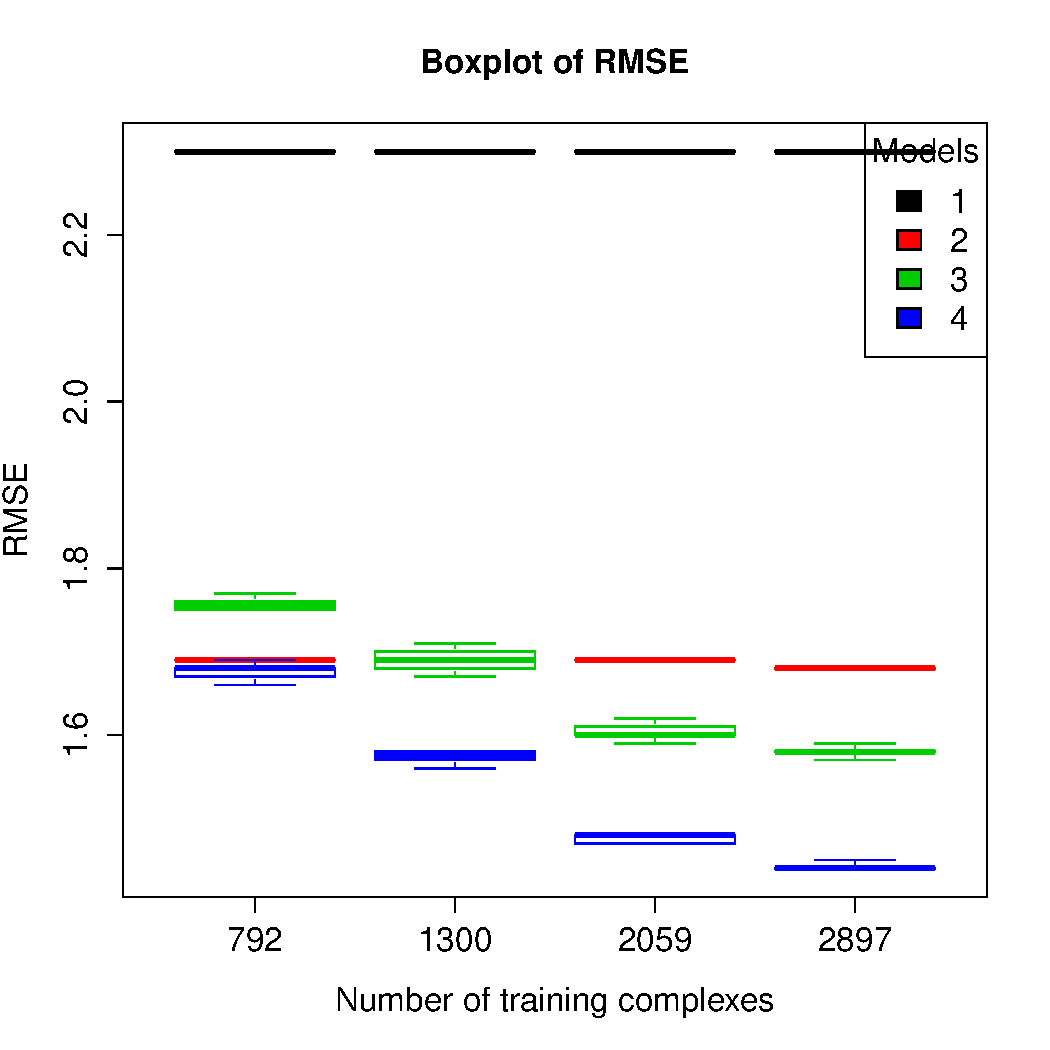
\includegraphics[width=0.48\linewidth]{../rfscore3/set-2-tst-rmse-boxplot.pdf}
}
\subfloat
{
  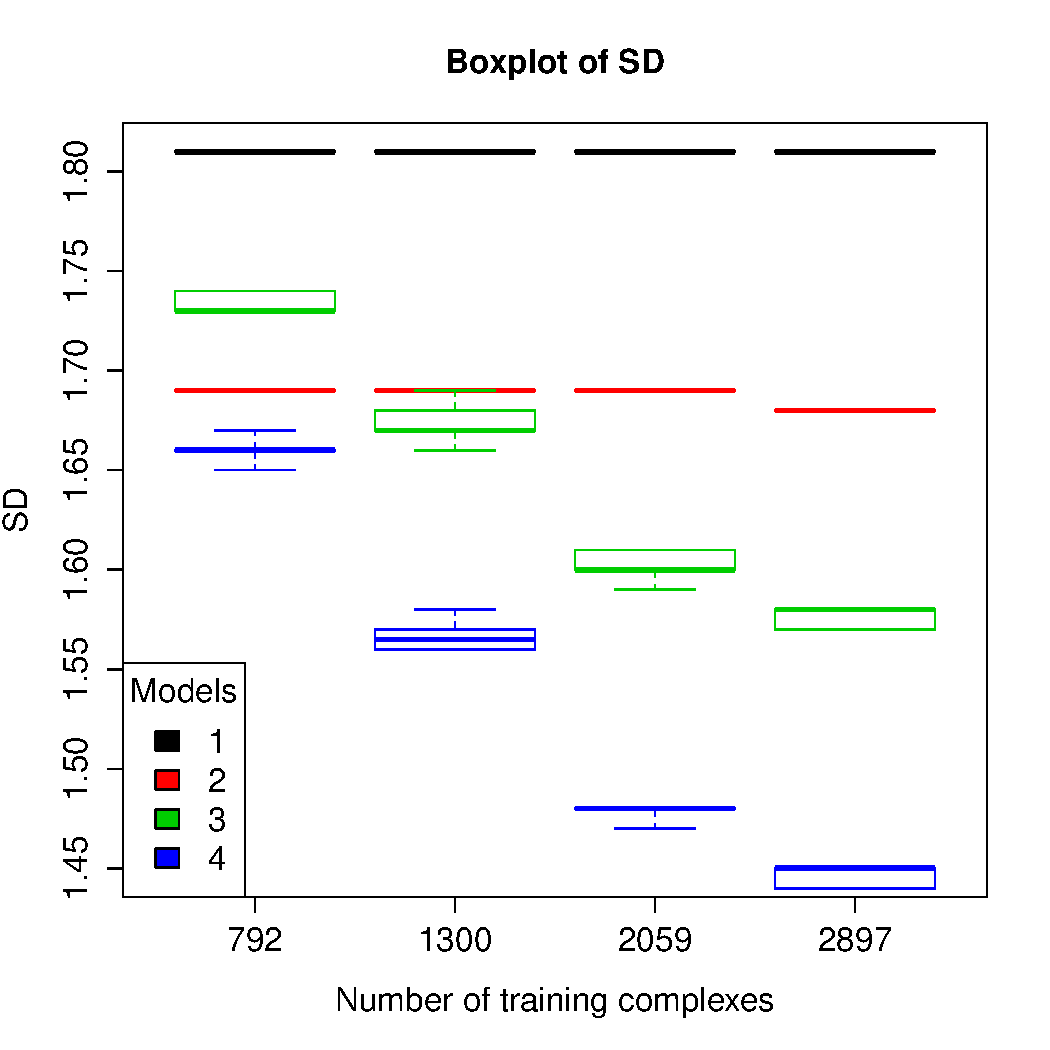
\includegraphics[width=0.48\linewidth]{../rfscore3/set-2-tst-sdev-boxplot.pdf}
}
\\
\subfloat
{
  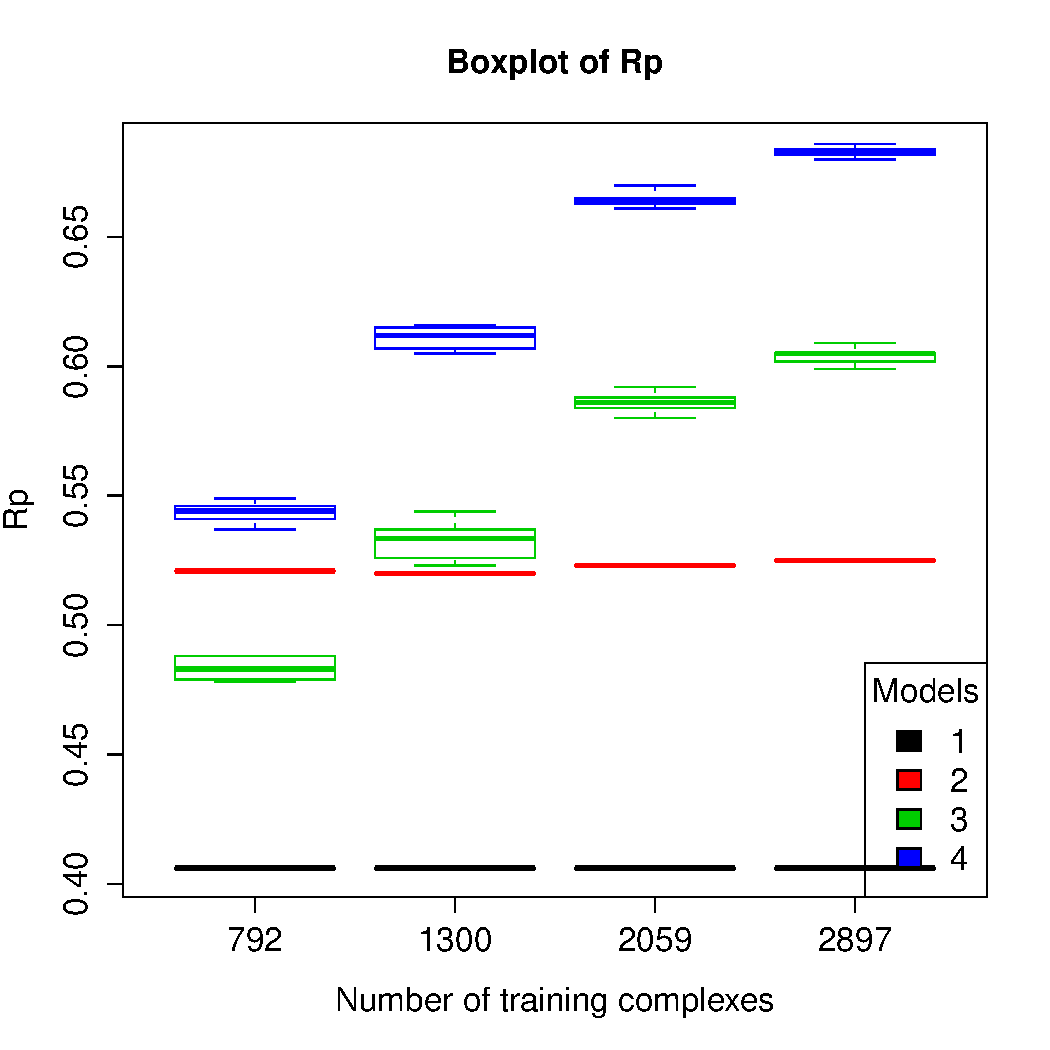
\includegraphics[width=0.48\linewidth]{../rfscore3/set-2-tst-pcor-boxplot.pdf}
}
\subfloat
{
  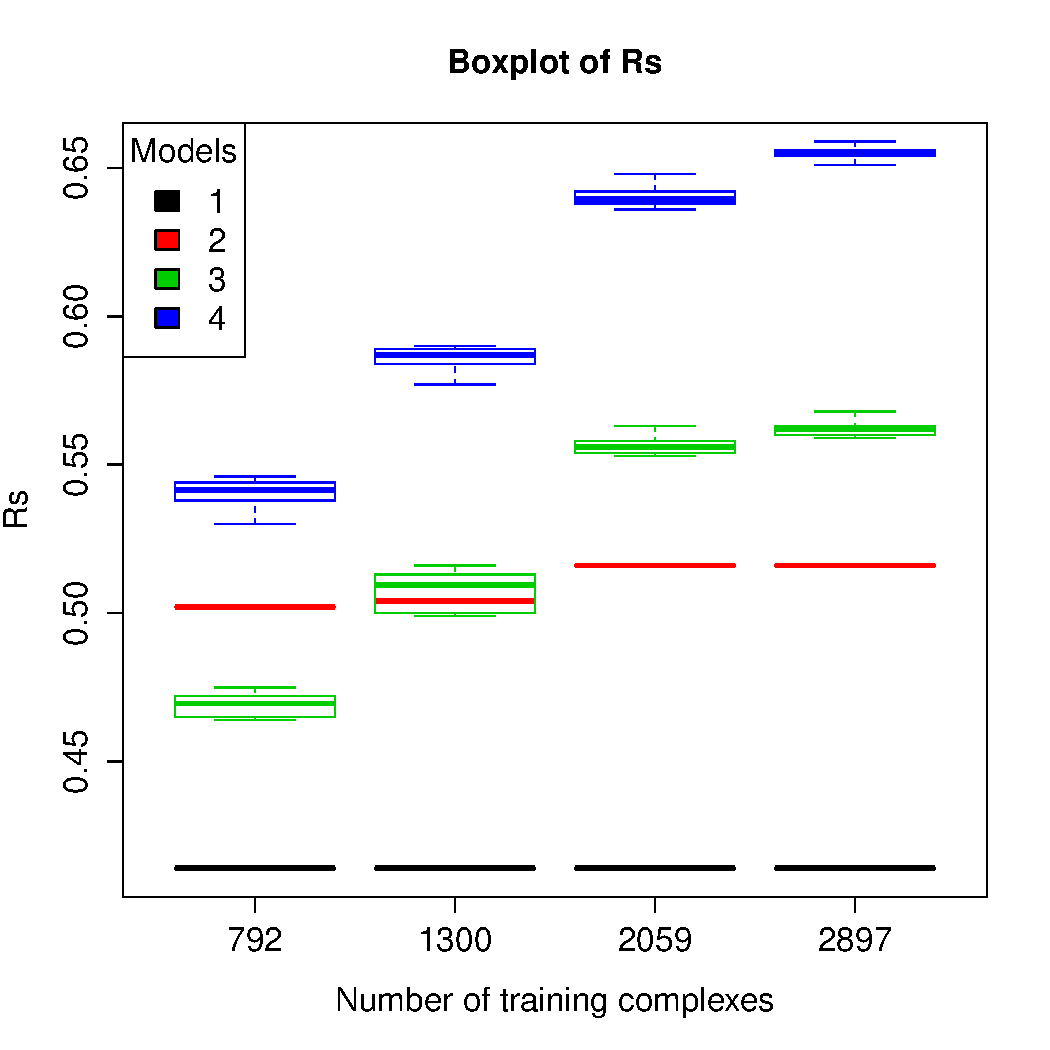
\includegraphics[width=0.48\linewidth]{../rfscore3/set-2-tst-scor-boxplot.pdf}
}
\caption{Performance in predicting binding affinity on the 382 new complexes in 2013 using training sets formed by the complexes known in 2002, 2007, 2010 and 2012.}
\label{rfscore3:set-2-tst-stat-boxplot}
\end{figure}

The second reason why machine-learning scoring functions perform so well is that RF is capable of effectively exploiting a more comprehensive set of structural features. This can be seen by comparing the performance of models 3 and 4, which only differ in that model 4 uses 36 features in addition to the 6 features used by model 3. Not only the difference in performance is substantial but grows as more data is available for training. This observation increases again the importance of using RF in the future.

The same conclusions are reached from this complementary view of performance: a non-parametric regression model performs better because it circumvents modelling assumptions and is capable of exploiting richer structural descriptions of the complex. For the training set with the lowest number of complexes, model 2 outperforms model 3, indicating that the additivity assumption of classical scoring functions was the best approach back in the days when few structures were available to calibrate the scoring function. It is also noteworthy that model 1 performs worse than model 2, which suggests that the nonlinear OLS used in Vina is not as suitable as MLR, at least for this crucial aspect of docking, i.e. scoring complexes. Note that model 1 represents the situation where the Vina's scoring function was used out of the box without retraining for each set, although here we have seen that improvements with data set size can only be gained by using the appropriate regression model.

\subsection{Machine-learning scoring functions can also be used to interpret docking results}

In addition to predicting binding affinity, the magnitude of the terms or features of a scoring function for a docking pose can be used to find out which the most important contributions to binding are. There are a number of approaches for this sensitivity analysis. In a chemical series, one can look at how the value of each feature correlates with measured binding affinity, the more important for binding being those obtaining a higher correlation. For a particular docking pose, one can multiply each feature with its weight to obtain the energetic contribution to binding of each feature. Because knowledge-based scoring functions typically have no weights, it has been claimed \citep{1372} that these can barely provide immediate physical interpretation of the results. In reality, one could also evaluate the scoring function for that pose with each feature set to zero in turn, with the features resulting in the largest variation in the predicted pKd value being the most important. This can also be easily implemented in machine-learning scoring functions to understand ligand binding.

Another potential issue is that the set of features may not be directly related to intermolecular interactions. This is not the case of model 3, which has the same six directly interpretable features as model 2 representing an empirical scoring function. Nevertheless, model 4 incorporates 36 additional features which are not directly interpretable. Before assessing whether this is a drawback, we should remember what interpretability is ultimately useful for. Often, the optimisation of ligand potency is carried out by synthesising derivatives that preserve important favourable interactions and reduce unfavourable interactions according to such interpretation. However, extracting knowledge from a docking pose using a less accurate scoring function to use the derived knowledge to optimise ligand potency is apparently less accurate than simply using the most accurate scoring function to score all possible derivatives in order to synthesise those that are predicted to be more potent. Therefore, rather than a drawback, we believe that circumventing the interpretability stage can be an advantage in structure-based optimisation.

\subsection{The applicability domain of the developed scoring functions}

The applicability domain of a regression model is given by the set of training data points and how they are represented. In consequence, models 2 and 3 have the same applicability domain and thus are expected to work well on the same types of small molecules and proteins. Model 4 is trained and tested on the same data sets and thus should have a similar applicability domain than models 2 and 3. However, because model 4 incorporates an additional set of features, so the data representation is different and thus the applicability domain is not exactly the same. It is important to note that these features encode neither the chemical structure of the ligand nor the sequence information of the protein. Therefore, there is no reason to think that its applicability domain is more restricted to the chemotypes and protein families in the training set any more than other scoring functions trained on the same data are.

\section{Conclusions}

We have seen that one can greatly improve Vina by circumventing its assumed functional form using RF as the regression model and expanding the set of features describing the complexes. The resulting machine-learning scoring functions have either the same or very similar applicability domain by construction. Furthermore, we have explained how these scoring functions could be also used to understand binding. However, we have also argued that extracting knowledge from the description that a scoring function provides of a docking pose is a suboptimal way to improve ligand binding, as the direct application of a more accurate scoring function on ligand derivatives should perform better. We have demonstrated that the tendency of RF-based scoring functions to overfit training data is not a limitation but instead a trait of these regression models which are robust to overfitting. Finally, we have also suggested that incorporating ligand- and protein-only properties into the scoring function is a promising path to future improvements.

Another big contribution of this study is the release of free software implementing RF::VinaElem so that it can be directly used by the large number of Vina users, and literally by all users after converting the file format to PDBQT using OpenBabel \citep{968} or AutoDock Tools \citep{596}. Given the large number of Vina users and the large increase in scoring accuracy achieved, we have trained the best of our models on the most comprehensive set of high-quality complexes (RF-Score-v3; RF::VinaElem trained on the 2959 complexes from 2013 refined set) and implemented it as easy-to-use free software that directly re-scores Vina-generated poses. Given its accuracy at ranking complexes, RF-Score-v3 should generally perform well on structure-based drug lead optimization.

Because classical scoring functions generally use MLR as the regression model and we have shown its inability to improve with larger sizes of structural data, we expect that the performance of any of these will be boosted by following the same procedure we have applied here to Vina. We therefore suggest developers modify their scoring functions accordingly so that users can enjoy a much higher predictive accuracy. Using non-parametric machine learning remains a largely unexplored approach to developing scoring functions. For example, the incorporation of ligand-only, protein-only and alternative intermolecular features, e.g. \citep{1303}, is still to be fully investigated.

The proposed PDBbind 2013 benchmark, effectively a blind test using four time-stamped training sets, has revealed that the performance difference between classical and machine-learning scoring functions will be larger as more structural data becomes publicly available in the future. These machine-learning scoring functions could include the very large number of experimentally determined structures that are continuously generated by the pharmaceutical industry and the academic institutes. Confidentiality is not be a problem because only the inter-molecular features and binding affinities of these structures are required to train scoring functions, from which it is impossible to decode the identity of either the targets or the bound molecules. It is important to note that this is a new opportunity because, as we have shown here, the regression model adopted by classical scoring functions would not be able to exploit new flood of data.

As usual, e.g. \citep{1313}, the performance of generic scoring functions has been assessed by measuring their ability to predict the binding affinities of diverse protein-ligand complexes. Given its accuracy at this task, RF-Score-v3 should generally perform well on structure-based drug lead optimization applications. We have however not yet investigated its ability to discriminate between binders and non-binders in virtual screening (VS) settings, as it is important to first study binding affinity prediction in isolation so as to avoid additional confounding factors such as true binders that might not bind to the assumed binding conformation or pocket as well as assumed non-binders that might be actually binding. This problem, known as enrichment, belongs to another dedicated study, as it has previously been the case \citep{977,1477}, mainly because additional research is required to find an optimal configuration of the scoring function, which might involve different features and training strategies. Since these issues are hence out the scope of this study, we are not making any claim about how RF-Score-v3 will compare to classical scoring functions on VS benchmarks. However, we expect that it will excel at VS because: 1) excellent prospective results have already been achieved with the less accurate RF-Score-v1 \citep{1281}, 2) pose generation error has typically a low impact on binding affinity prediction \citep{1362}, 3) accurate ranking by the affinity of true binders is a necessary condition for top VS performance, and 4) non-binders are nothing but extremely weak binders whose low affinity should be best predicted by RF-Score-v3. In fact, machine-learning scoring functions have already demonstrated substantial improvements over classical scoring functions on VS benchmarks \citep{1476}.

\section{Availability}

RF-Score-v3 is free and open source under Apache License 2.0. The source code is available at https://github.com/HongjianLi/RF-Score. The precompiled 64-bit executables for Linux and Windows, a README file for operating instructions, a prebuilt RF file, a sample protein file and a sample ligand file in PDBQT format are available at http://istar.cse.cuhk.edu.hk/rf-score-3.tgz.

\section{Future works}

The current study can be extended in multiple aspects. From the perspective of training data compositions, leave-cluster-out cross validation (LCOCV) \citep{774} is becoming a popular validation method in evaluating scoring function performance of predicting binding affinity of truly new protein targets. \citep{1423} compares confirmed inactive and randomly selected compounds as negative training examples in support vector machine-based virtual screening. \citep{1404} analyzes the influence of negative training set size on machine learning-based virtual screening.

From the perspective of new benchmarks, the well known PDBbind benchmark has recently been updated to CASF-2013 \citep{1426}, and 20 scoring functions, most of which are implemented in mainstream commercial software, have been evaluated in terms of ``scoring power" (binding affinity prediction), ``ranking power" (relative ranking prediction), ``docking power" (binding pose prediction), and ``screening power" (discrimination of true binders from random molecules) \citep{1411}.

From the perspective of features, the DRAGON 6 software \citep{1478}, available at http://www.talete.mi.it/, can calculate 4885 molecular descriptors. PaDEL-descriptor \citep{1479} and QuBiLS-MIDAS \citep{1400} are free software for molecular
descriptors computation. It is also possible to borrow the ideas of UFSRAT \citep{1436} and USRCAT \citep{1331} and generate features from subsets of atoms.

From the perspective of regression models, the random generalized linear model (RGLM) has recently been proposed \citep{1377} as a highly accurate and interpretable ensemble predictor, and subsequently evaluated in predicting the status of COPD (chronic
obstructive pulmonary disease) \citep{1418}.

From the perspective of applications, it is interesting to see an analogous scoring function tailored to the enrichment problem of discriminating between binders and non-binders, as well as scoring functions specific to protein families. Moreover, like T-PioDock \citep{1399}, machine-learning scoring functions can be applied to protein-protein docking.

\chapterend
